\documentclass[conference]{IEEEtran}
\IEEEoverridecommandlockouts
\usepackage[T1]{fontenc}
\usepackage[utf8]{inputenc}
\usepackage{cite}
\usepackage{amsmath,amssymb}
\usepackage{graphicx}
\usepackage{booktabs,tabularx,array}
\usepackage{xurl}
\usepackage{algorithm}
\usepackage[noend]{algpseudocode}
\usepackage{textcomp}
\def\BibTeX{{\rm B\kern-.05em{\sc i\kern-.025em b}\kern-.08em T\kern-.1667em\lower.7ex\hbox{E}\kern-.125emX}}

\begin{document}

\title{Detecting Unsupported Claims in RAG Answers with Calibrated Cheap Scoring and Selective Verification}

\author{\IEEEauthorblockN{Iqra Farooq}
\IEEEauthorblockA{\textit{Department of Computer Science}\\ \textit{National University of Computer and Emerging Sciences (FAST-NUCES)}\\ Islamabad, Pakistan\\ i267839@isb.nu.edu.pk}}

\maketitle

\begin{abstract}
Retrieval-augmented generation (RAG) grounds large language models in retrieved evidence, yet generated answers still contain claims that the evidence does not support. Verifying every claim with an expensive model is accurate but costly. We propose an adaptive claim-level verifier that estimates a calibrated probability of evidence support for each claim from cheap signals (similarity, lexical and entity/number coverage, and contradiction cues from a small natural-language-inference (NLI) model) and escalates only uncertain or disagreeing claims to a stronger verifier, with thresholds chosen by an explicit cost--quality objective. On the full HaluBench test set (10,422 answers), the verifier proves decisive: a large NLI model raises uniform verification from F1 0.669 to 0.753 (AUROC 0.816), ahead of HHEM-2.1 (0.695) and MiniCheck (0.657). At matched budgets, uncertainty-based escalation outperforms random and lowest-support escalation (F1 0.723 vs. 0.680 and 0.611 at 30\% of calls) and matches uniform verification with 75\% of the calls, whereas a disagreement signal adds nothing. On 1,400 HotpotQA claims that require two documents, premise coverage is the main bottleneck (AUROC 0.785 with top-4 sentences vs. 0.927 with gold evidence). We also reproduce a recent faithfulness benchmark and show that the gap to its printed retrieval scores stems mainly from question-scoped document identifiers that count duplicate sentences as non-relevant.
\end{abstract}

\begin{IEEEkeywords}
Retrieval-augmented generation, claim-level verification, faithfulness hallucination, hallucination detection, uncertainty-gated verification
\end{IEEEkeywords}

\section{Introduction}

Large language models (LLMs) now answer questions inside search engines, assistants and enterprise tools, so their errors reach users directly. Hallucination, the generation of fluent but nonfactual or unfaithful content, is therefore a central reliability problem for information systems~\cite{huang_tois}. Retrieval-augmented generation (RAG) conditions the model on documents retrieved at inference time and has become the standard remedy; recent surveys treat it as a general knowledge-oriented paradigm~\cite{cheng_tois} and organize its methods by pipeline stage~\cite{huang_csur}; surveys written from the information-retrieval~\cite{zhu_tois} and trustworthiness~\cite{ni_csur} perspectives reach the same conclusion.

Multi-hop questions expose the limits of this remedy. An answer must combine facts from several documents, which vanilla RAG handles poorly because it does not model relationships across documents~\cite{peng_tois}. Retrieval quality is also not the same as faithfulness. A systematic benchmark of sparse, dense and hybrid retrieval with three open-weight LLMs found that hybrid retrieval raised answer accuracy for the two larger models but also raised their hallucination rates, for example from 9.34\% to 16.00\% for Qwen3-4B on HotpotQA~\cite{mala_ml}. Models used better evidence more often, but not always faithfully.

Existing work attacks the problem from three directions. Retrieval-side methods improve the evidence before generation through query planning and structured evidence extraction~\cite{huang_tkdd}, knowledge-graph-guided retrieval with a hypothesis-and-verification loop~\cite{yuan_jksu}, question decomposition~\cite{linders_ai}, utility-driven re-ranking~\cite{wu_ml} pre-generation passage gates~\cite{kirubavathi_sr} or retrieval-quality prediction~\cite{sinha_tois}. Output-side methods verify generated content: atomic-fact verification against a knowledge source~\cite{min_factscore}, sentence-level NLI~\cite{laban_summac}, trained factual-consistency models~\cite{zha_alignscore},~\cite{tang_minicheck},~\cite{vectara_hhem}, citation validation~\cite{qian_vericite} and claim-level self-verification with calibration~\cite{pal_dai}. A third line spends computation selectively: retrieval is triggered when the generator is unsure~\cite{jiang_flare}, consistency is checked by sampling several answers~\cite{manakul_selfcheck}, and mid-confidence passages receive an extra audit~\cite{kirubavathi_sr}.

Each ingredient of our method therefore exists on its own: claim-level verification~\cite{min_factscore},~\cite{tang_minicheck}, calibration~\cite{pal_dai} and selective computation~\cite{jiang_flare},~\cite{kirubavathi_sr}. What is missing is their combination for one specific decision, namely \textit{which generated claims are worth an expensive check against the retrieved evidence}. Three gaps follow. (G1) Claim verifiers spend the same effort on every claim~\cite{min_factscore},~\cite{tang_minicheck},~\cite{pal_dai},~\cite{qian_vericite}, while existing selective methods decide from the generator's own confidence~\cite{jiang_flare},~\cite{manakul_selfcheck} or act on passages before generation~\cite{kirubavathi_sr}, not on output claims against evidence. (G2) The intermediate and final claims of multi-hop answers are rarely checked against evidence composed from several documents; multi-hop methods act on retrieval~\cite{huang_tkdd},~\cite{yuan_jksu} or require trained reward models~\cite{sun_rearter}, and consistency models score a claim against fixed chunks~\cite{zha_alignscore},~\cite{tang_minicheck}. (G3) Faithfulness is usually evaluated per answer or per citation and without cost: the base benchmark labels whole answers~\cite{mala_ml}, and correct citations can still be unfaithful~\cite{wallat_ictir}. Accordingly, the objectives are to (O1) reproduce the base pipeline and measure unsupported claims across retrievers and generators, (O2) design and evaluate an adaptive claim verifier, and (O3) compare adaptive, cheap-only and uniform verification, and established detectors, in detection quality and cost.

The study addresses three research questions. \textbf{RQ1:} How often do RAG answers to multi-hop questions contain unsupported claims under different retrievers and generators, and how does this relate to answer-level judge labels? \textbf{RQ2:} How accurately can an adaptive claim verifier, which escalates only uncertain claims, detect unsupported answers compared with cheap-only verification, uniform full verification and existing factual-consistency detectors? \textbf{RQ3:} How much verification cost (verifier calls and time) does adaptive escalation save, and at what change in detection quality? RQ2 and RQ3 are answered on the full HaluBench test set and on multi-hop HotpotQA claims; RQ1 is addressed in part: Qwen3-4B answers to 1,200 HotpotQA questions were generated under sparse, dense and hybrid retrieval, while their judge labelling and verification remain future work.

We propose an adaptive claim-level evidence verifier (Fig. 1). Its contributions are: (i) a calibrated cheap support model that combines embedding similarity, lexical and entity/number coverage and contradiction-sensitive features, trained on answer- or claim-level labels; (ii) a gate that escalates uncertain claims, or claims on which two cheap signals disagree, with thresholds chosen by an explicit cost--quality objective and compared with random and confidence-based escalation at matched budgets; (iii) top-$m$ and evidence-chain premises for claims that need several documents, evaluated on multi-hop claims with exact labels; (iv) a diagnosis of why NLI verification failed in our first version and a stronger verifier; and (v) a reproduction of the base benchmark~\cite{mala_ml}, including controlled experiments that explain the gap to its printed retrieval scores. Section II reviews related work, Section III describes data and method, Section IV reports the experiments, Section V discusses the findings, and Section VI concludes.

\section{Related Work}

Research on hallucination in retrieval-augmented systems has converged on a shared vocabulary but not on a shared remedy. The field now distinguishes factuality errors, where an answer contradicts world knowledge, from faithfulness errors, where it departs from the evidence the system was given, and broad overviews of the area consistently name two unresolved issues: verification at the granularity of individual claims, and the computational cost that such verification incurs. Both issues are acknowledged far more often than they are measured, and that imbalance frames the present study.

\begin{table*}[t]
\centering
\caption{Comparison of verification method families: mechanism, compared unit and evidence, cost, main limitation and typical evaluation data. LLM: large language model; NLI: natural language inference; QA: question answering.}
\label{tab:t1}
\footnotesize
\setlength{\tabcolsep}{3pt}
\renewcommand{\arraystretch}{1.12}
\begin{tabularx}{\textwidth}{>{\raggedright\arraybackslash\hsize=0.953\hsize}X>{\raggedright\arraybackslash\hsize=1.094\hsize}X>{\raggedright\arraybackslash\hsize=1.059\hsize}X>{\raggedright\arraybackslash\hsize=0.882\hsize}X>{\raggedright\arraybackslash\hsize=1.059\hsize}X>{\raggedright\arraybackslash\hsize=0.953\hsize}X}
\toprule
\textbf{Method family} & \textbf{Verification mechanism} & \textbf{Unit and evidence} & \textbf{Cost per answer} & \textbf{Main limitation} & \textbf{Typical evaluation data} \\
\midrule
Atomic-fact verification & LLM decomposition, retrieval and LLM or NLI check & Atomic fact vs. knowledge source & One LLM call per fact & Needs a knowledge source; uniform effort & Biographies, long-form text \\
Sentence-pair NLI & NLI on sentence pairs, aggregated & Sentence vs. document sentences & NLI on all sentence pairs & Granularity mismatch; no premise composition & Summarization consistency \\
Trained consistency models & Alignment or consistency classifier & Sentence vs. context chunks & One pass per chunk and sentence & Uniform; claims checked in isolation & Summarization, dialogue, grounding benchmarks \\
Sampling consistency & Agreement among sampled answers & Sentence vs. other samples & N extra generations & No evidence; costly & Biography generation \\
Confidence-triggered retrieval & Retrieve when the generator is unsure & Next sentence; retrieved documents & Extra retrieval and regeneration & Gates retrieval, not verification & Multi-hop and long-form QA \\
Probing with calibration & Repeated probing, calibrated risk & Claim vs. model's own probes & Several probes per claim & No retrieved evidence; uniform & Truthfulness QA \\
Citation validation & Evidence check per citation & Citation vs. cited passages & One check per citation & Citation-level; uniform & RAG QA with citations \\
Pre-generation gating & Passage gate; audit if mid-confidence & Passage, before generation & Audit of uncertain passages & Generated claims are not checked & Hallucination QA (small samples) \\
Process reward models & Trained step-level reward models & Reasoning step & Reward-model passes per step & Requires training data & Multi-step reasoning QA \\
LLM-judge benchmarking & LLM judge of the whole answer & Answer vs. ground truth & One judge call per answer & Answer-level; cost not studied & HotpotQA, HaluBench \\
\textbf{This work} & \textbf{Calibrated cheap signals; escalate uncertain or disagreeing claims} & \textbf{Claim (incl. reasoning steps) vs. multi-sentence or chained evidence} & \textbf{Verifier only for escalated claims} & \textbf{Limited by the cheap stage and premise coverage} & \textbf{HaluBench, HotpotQA} \\
\bottomrule
\end{tabularx}
\end{table*}

A first body of work tries to prevent unfaithful answers by improving the evidence before the language model writes anything. Approaches in this line plan the retrieval of multi-hop evidence, traverse knowledge graphs and retrieve again when a bridge fact is missing, decompose complex questions into simpler ones, re-rank passages by their usefulness for a correct and faithful answer, or reject passages that fail relevance and consistency checks before generation. Some predict retrieval quality from cheap post-retrieval signals. These methods are valuable because better evidence raises accuracy, yet they share a structural blind spot: they decide what the model reads, not whether what it finally writes is supported. A model that receives perfect evidence can still combine it incorrectly, and the base benchmark reproduced here shows exactly this pattern, with stronger retrieval raising accuracy and hallucination together.

A second body of work therefore verifies the output itself. Its methods differ mainly in the unit they check and the evidence they check it against. Decomposing long text into atomic facts and checking each against a knowledge source is precise, but it spends one language-model call per fact and assumes that the relevant facts can be retrieved. Applying sentence-level natural language inference to every pair of evidence and output sentences showed that inference models work only at the right granularity, at a cost that grows with the product of the two lengths. Trained alignment and consistency classifiers score a claim against chunks of the context and approach the quality of much larger checkers at a fraction of their cost, and citation-validation methods ask whether cited passages really support the statements they are attached to; a related observation is that correct attributions can still be unfaithful. Across this line, two habits recur: every claim receives the same verification effort, and evaluation is dominated by summarization and grounding benchmarks rather than multi-hop question answering, where a single claim may require evidence from several documents.

A third body of work spends computation selectively, which is the idea the present method builds on. Generators can trigger new retrieval when their own next-sentence confidence is low; hallucinations can be detected by sampling several answers and measuring their agreement; claim risk can be estimated by repeated probing and then calibrated; passages of intermediate confidence can be sent to an external audit before generation; and reasoning steps can be scored by trained process-reward models. These approaches demonstrate that uncertainty is a useful signal for allocating effort, but they compute it from the generator's own behaviour, apply it before generation, or require additional generations and trained reward models. None of them uses signals computed against the retrieved evidence to decide which generated claims deserve an expensive check.

Table I summarizes the method families along the four dimensions that matter for this decision: the verification mechanism, the unit and evidence that are compared, the cost per answer, and the main limitation, together with the data on which each family has typically been evaluated. The comparison shows that the field has developed strong verifiers that are applied uniformly and selective mechanisms that are applied to retrieval or to the generator, but that the two have not been joined at the level of output claims and retrieved evidence. The method proposed here occupies that gap: it decides per claim, from cheap evidence-based signals, whether the expensive verifier is needed, and it is evaluated on detection quality and cost together, against random and confidence-based escalation at matched budgets.

\section{Materials and Methods}

\subsection{Research Datasets and Data Preparation}

\textbf{HotpotQA}~\cite{yang_hotpot} (distractor setting, CC BY-SA 4.0, Hugging Face \textit{hotpotqa/hotpot\_qa}) contains 90,447 training and 7,405 validation questions. Each question comes with ten Wikipedia paragraphs, two of which are supporting, and with sentence-level supporting facts. Following the base repository~\cite{mala_ml}, every sentence of the supporting paragraphs becomes one document in a pooled corpus, identical sentences are stored once after lower-casing and whitespace normalization, and the annotated supporting sentences are the relevant documents of each question. Annotations that point past the end of a paragraph are discarded. Retrieval is evaluated on the training split as in the base paper. For the end-to-end experiment, 1,200 training questions sampled with seed 42 (as in the base repository) are searched against the full corpus with a sparse (BM25), a dense (Contriever) and a hybrid retriever (linear interpolation with reranking), and answered from the top-5 sentences. For a controlled multi-hop test, 1,000 validation questions are sampled; for each we build one supported claim, ``The answer to the question $q$ is $a$.'' with the gold answer, and one unsupported claim with a hard wrong answer: the other entity of a comparison question, the flipped yes/no, a perturbed number, the bridge entity of a bridge question, or the title of a distractor paragraph. Their evidence is the question's ten paragraphs (two supporting, eight distractors), so verifying the claim requires the two supporting documents and exact labels are available.

\textbf{HaluBench} (Hugging Face \textit{PatronusAI/HaluBench}) contains about 15,000 context--question--answer triplets from six sources (HaluEval, DROP, RAGTruth, FinanceBench, PubMedQA and CovidQA), each labelled as faithful (PASS) or hallucinated (FAIL)~\cite{mala_ml}. Rows with missing fields and exact duplicates are removed, leaving 14,888 answers. Unlike our first version, which used the 1,200-answer sample of~\cite{mala_ml}, all of them are used: a development set (30\%, 4,466 answers, stratified by source) is used only for fitting calibrators and selecting thresholds, and a test set (70\%, 10,422 answers) for all reported results. HaluEval contributes two thirds of the rows and has short, easy passages, so we also report the F1 averaged over the six sources (macro-F1). Download links and access dates for all datasets are listed in the Data and Code Availability section.

\begin{table*}[t]
\centering
\caption{Datasets, partitions and their role.}
\label{tab:t2}
\footnotesize
\setlength{\tabcolsep}{3pt}
\renewcommand{\arraystretch}{1.12}
\begin{tabularx}{\textwidth}{>{\raggedright\arraybackslash\hsize=1.000\hsize}X>{\raggedright\arraybackslash\hsize=0.833\hsize}X>{\raggedright\arraybackslash\hsize=0.750\hsize}X>{\raggedright\arraybackslash\hsize=0.722\hsize}X>{\raggedright\arraybackslash\hsize=1.694\hsize}X}
\toprule
\textbf{Dataset} & \textbf{Split / sample} & \textbf{Size} & \textbf{Labels} & \textbf{Use in this study} \\
\midrule
HotpotQA distractor~\cite{yang_hotpot} & train & 90,447 questions & Supporting sentences & Retrieval reproduction (Tables 1 and 3 of~\cite{mala_ml}) \\
HotpotQA distractor~\cite{yang_hotpot} & train, 1,200 sampled & 1,200 questions $\times$ 3 retrievers & Gold answers & End-to-end generation with Qwen3-4B (E1); verification is future work \\
HotpotQA multi-hop claims & validation, 1,000 sampled & 2,000 claims (dev 600, test 1,400) & Exact (by construction) & Premise construction, claim-level calibration \\
HaluBench & all six sources & 14,888 answers (dev 4,466, test 10,422) & PASS / FAIL & Verifier, gate, ablations (E2) \\
Pooled sentence corpus & from supporting paragraphs & 338,582 sentences & --- & Retrieval index \\
\bottomrule
\end{tabularx}
\end{table*}

A representative HotpotQA question is \textit{``Which magazine was started first, Arthur's Magazine or First for Women?''}; answering it requires the founding years from two different articles, so a correct answer contains at least two intermediate claims that are each supported by a different sentence. This is the kind of claim the multi-sentence and evidence-chain premises of Section III-C are designed to verify.

\subsection{Problem Formulation}

Let $q$ be a question, $R$ a retriever returning the top-$k$ evidence sentences $D$ = $R$($q$), and $G$ a frozen generator producing an answer $a$ = $G$($q$, $D$). A claim extractor $E$ maps the answer to claims $E$($a$) = \{$c_{1}$, \ldots{}, $c_{n}$\}; short answers are turned into hypotheses $h_{i}$ by attaching the question. Each claim has an unobserved label $y_{i}$ $\in$ \{0, 1\}, with $y_{i}$ = 1 if $D$ does not support $c_{i}$. The task is to predict $z_{i}$ for every claim and the answer-level label $z$($a$) = max\textsubscript{$i$} $z_{i}$, while limiting the number of calls to an expensive verifier. With $C$($\theta$) the number of verifier calls under gate threshold $\theta$ and $C_{\mathrm{full}}$ the number under uniform verification, thresholds are chosen on the development set $D_{\mathrm{dev}}$ by

\begin{equation}
(\theta^*,\tau^*)=\arg\min_{\theta,\tau}\bigl[1-\mathrm{F1}_{\mathrm{dev}}(\theta,\tau)\bigr]+\lambda\cdot\frac{C(\theta)}{C_{\mathrm{full}}}
\label{eq:e1}
\end{equation}

where F1 is computed for unsupported answers, $\tau$ is the verifier threshold and $\lambda$ $\ge$ 0 sets the price of a call. \textbf{Assumptions:} support is judged against the retrieved context only (faithfulness, not world truth); claims are verified independently; the generator is not modified. Eq. (1) encodes gap G1 (cost) at the claim granularity of G2, and evaluation under several retrieval conditions addresses G3.

\subsection{Proposed Methodology}

\textit{Overview:} The verifier runs after generation and does not change the retriever or generator. It has four stages: claim extraction, cheap support scoring, uncertainty gating and full verification (Fig. 1).

\begin{figure*}[t]
\centering
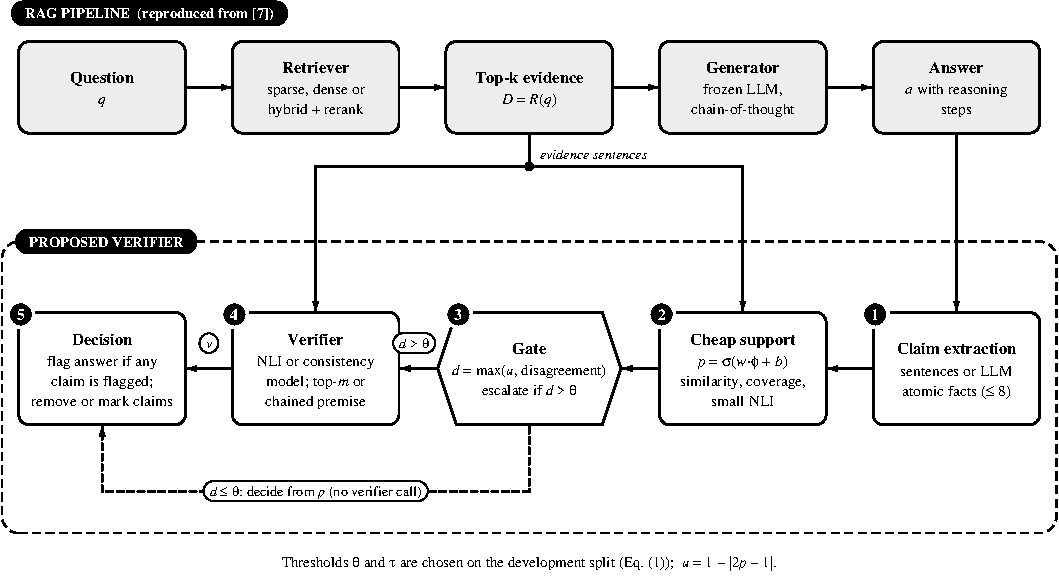
\includegraphics[width=\textwidth]{figures/fig1.pdf}
\caption{Workflow of the proposed method. The upper row (grey) is the reproduced RAG pipeline of~\cite{mala_ml}; the dashed region is the proposed verifier, whose stages are numbered in execution order. Confident claims bypass the verifier (dashed path).}
\label{fig:f1}
\end{figure*}

\textit{Claim extraction:} The output, including its reasoning steps, is split into sentences; step labels, meta-reasoning (e.g., statements about the task) and refusals are removed, duplicates are dropped and at most eight claims are kept. A bare short answer (five words or fewer) becomes the hypothesis ``The answer to the question $q$ is $c$.'' so that it can be checked by entailment. Keeping step sentences is deliberate: in multi-hop answers the bridge facts appear there. The rule-based extractor works at sentence level: a sentence that states several facts stays one claim, which the verifier must then entail as a whole. As an alternative we use LLM-based decomposition into atomic facts, in the style of~\cite{min_factscore}, with an open-weight chat model (Qwen2.5-7B-Instruct) instructed to output one self-contained fact per line, resolve pronouns and drop statements about the task; Section IV compares both extractors and measures how often the eight-claim cap is reached.

\textit{Cheap support score:} Let $U$($D$) be the evidence sentences and $e$($\cdot$) a normalized sentence embedding. For claim $c_{i}$ with hypothesis $h_{i}$, four features are computed:

\begin{equation}
\begin{aligned}s_{\max}&=\max_{u\in U(D)}\cos\bigl(e(h_i),e(u)\bigr),\\ s_{\mathrm{top3}}&=\text{mean of the three largest similarities}\end{aligned}
\label{eq:e2}
\end{equation}

\begin{equation}
\begin{aligned}c_{\mathrm{lex}}&=\frac{|W(c_i)\cap V(D)|}{|W(c_i)|},\\ c_{\mathrm{key}}&=\frac{|K(c_i)\cap V(D)|}{|K(c_i)|}\end{aligned}
\label{eq:e3}
\end{equation}

where $W$($\cdot$) are content words, $K$($\cdot$) are numbers and capitalized entity tokens, and $V$($D$) is the vocabulary of the evidence (a coverage is 1 when the set is empty). Entity and number coverage targets the most common hallucinations in HaluBench, swapped entities and altered numbers. These features measure overlap, not support: a claim can repeat the entities and numbers of the evidence and still state the opposite. We therefore add four contradiction-sensitive features: the entailment and contradiction probabilities $e_{\mathrm{small}}$, $c_{\mathrm{small}}$ of a small NLI cross-encoder (MiniLM, 6 layers) that reads only the single most similar evidence sentence, a negation-mismatch indicator (negation in exactly one of claim and best sentence), and the share of the claim's numbers that do not occur in the evidence. With $\phi_{i}$ the standardized vector of the four original features (original method) or of all eight (revised method), the calibrated support probability is

\begin{equation}
p_i=\sigma\bigl(w^{\top}\phi_i+b\bigr)
\label{eq:e4}
\end{equation}

\textit{Uncertainty gate:} The uncertainty of a claim is $u_{i}$ = 1 $-$ |2$p_{i}$ $-$ 1|, which is 0 when the cheap model is certain and 1 when $p_{i}$ = 0.5; for a binary decision this is the same as escalating the claims with the lowest confidence. The claim is escalated ($g_{i}$ = 1) if $u_{i}$ $>$ $\theta$. Setting $\theta$ = 1 never escalates, which gives cheap-only verification (B1). Setting $\theta$ = 0 escalates every claim with $u_{i}$ $>$ 0, i.e., every claim except those whose calibrated probability is exactly 0 or 1; it is therefore close to, but not identical with, uniform verification, which is run separately as baseline B2 and escalates every claim. A confidently wrong cheap prediction ($p_{i}$ near 0 or 1) bypasses this gate. The revised method therefore also escalates claims on which two independent support signals disagree, the calibrated probability and the small NLI model:

\begin{equation}
\begin{aligned}d_i&=\max\Bigl(u_i,\;\Bigl|p_i-\frac{1+e_{\mathrm{small}}-c_{\mathrm{small}}}{2}\Bigr|\Bigr),\\ g_i&=\mathbf{1}[d_i>\theta]\end{aligned}
\label{eq:e5}
\end{equation}

\textit{Full verifier and premise construction:} For an escalated claim the verifier reads a premise $P_{i}$ built from the evidence. The original method concatenates the $m$ = 4 evidence sentences most similar to $h_{i}$, restored to their original order (top-$m$). Since the most similar sentences need not form a reasoning chain, we also build a two-hop \textit{evidence chain}: hop 1 is the sentence most similar to the claim; hop 2 is the sentence, from a different document when document boundaries are known, that maximizes similarity to the claim plus 0.5 times its overlap with the \textit{bridge terms} of hop 1 (its entities and content words that are not in the claim); one further similar sentence is added. The verifier is either an NLI cross-encoder, $v_{i}$ = $P_{\mathrm{NLI}}$(entailment | $P_{i}$, $h_{i}$), or a factual-consistency model (MiniCheck~\cite{tang_minicheck}, HHEM-2.1~\cite{vectara_hhem}) that reads the full passage in chunks that fit its input, with the maximum over chunks as support score. The decision and the answer-level risk are

\begin{equation}
\begin{aligned}z_i&=g_i\,\mathbf{1}[v_i<\tau]+(1-g_i)\,\mathbf{1}[p_i<0.5],\\ r(a)&=1-\min_i\bigl[g_iv_i+(1-g_i)p_i\bigr]\end{aligned}
\label{eq:e6}
\end{equation}

\textbf{Algorithm 1} summarizes inference.

\begin{algorithm}[t]
\caption{Adaptive claim-level verification (inference for one answer)}
\label{alg:verify}
\begin{algorithmic}[1]
\Require question $q$, evidence $D$, answer $a$; calibrator $(w,b)$; thresholds $\theta,\tau$; premise rule; verifier $V$
\State $\{c_i\}\gets E(a)$; \ $h_i\gets\mathrm{hypothesis}(c_i,q)$
\For{each claim $i$}
  \State compute $\phi_i$ (Eqs.~(2)--(3), small-NLI and mismatch features)
  \State $p_i\gets\sigma(w^{\top}\phi_i+b)$; \ $d_i$ by Eq.~(5) (original method: $d_i=u_i$)
  \If{$d_i\le\theta$}
    \State $z_i\gets\mathbf{1}[p_i<0.5]$ \Comment{no verifier call}
  \Else
    \State $P_i\gets$ premise (top-$m$, evidence chain or passage chunks)
    \State $v_i\gets V(P_i,h_i)$; \ $z_i\gets\mathbf{1}[v_i<\tau]$
  \EndIf
\EndFor
\State \Return $z(a)=\max_i z_i$, risk $r(a)$ by Eq.~(6), claim report $\{(c_i,p_i,g_i,v_i,z_i)\}$
\end{algorithmic}
\end{algorithm}

\textit{Training and optimization:} No language model is fine-tuned. Only the calibrator is learned: $w$ and $b$ minimize the L2-regularized logistic loss. In the original method its training examples are the claims of single-claim development answers, whose claim label equals the answer label; this creates a mismatch, since the calibrator is then applied to the claims of multi-claim answers. We therefore also train it on genuine claim-level labels: exact labels for the HotpotQA multi-hop claims, and, for HaluBench, labels from an open-weight LLM judge (Qwen2.5-7B-Instruct) for 900 sampled claims, with 150 exported for manual annotation. $\tau$ is chosen on the development set to maximize the F1 of uniform verification, and $\theta$ by Eq. (1) over $\theta$ $\in$ \{0, 0.025, \ldots{}, 1\} $\cup$ \{0.99, 0.995, 0.999\} with $\lambda$ = 0.3; Section IV also reports the complete trade-off over $\theta$ and $\lambda$.

\textit{Inference and execution:} At test time the cheap stage needs one embedding pass over the evidence sentences and the claims and one small-NLI pass per claim on a single sentence; only escalated claims are sent to the verifier, in one batch per answer. The output is the answer with unsupported claims removed or flagged, plus a per-claim report.

\textit{Technical novelty and justification:} Claim verifiers~\cite{min_factscore},~\cite{zha_alignscore},~\cite{tang_minicheck} check every claim with the same model, and selective methods decide from the generator's confidence~\cite{jiang_flare},~\cite{manakul_selfcheck} or act on passages before generation~\cite{kirubavathi_sr}. Here the decision to spend the verifier is made per output claim, from signals computed against the retrieved evidence, and it escalates both uncertain claims and claims on which independent signals disagree (G1). The unit is the generated claim, including intermediate reasoning claims, checked against a multi-sentence or chained premise (G2), without training the generator~\cite{sun_rearter} or the verifier. Cost and detection quality are reported jointly, at matched budgets against random and confidence-based escalation, and across sparse, dense and hybrid retrieval (G3).

\section{Experimental Results and Discussion}

\subsection{Experimental Setup and Implementation}

Experiments run on free Kaggle instances with two NVIDIA Tesla T4 GPUs (15 GB each) and 31 GB RAM, with Python 3, PyTorch, Hugging Face Transformers, sentence-transformers, scikit-learn, SciPy and pytrec\_eval. All settings are in one configuration file, the seed is 42 everywhere, decoding is greedy, and judge responses are cached, so every run is repeatable. Three experiments are run. \textbf{E1} reproduces the base paper: retrieval on 10,000 training questions, an investigation of the gap to the printed values, and end-to-end generation on 1,200 questions with a sparse, a dense and a hybrid retriever. \textbf{E2} evaluates all verifier variants on the full HaluBench test set (10,422 answers), including matched-budget comparisons, ablations, error analyses and claim-level labels. \textbf{E3} tests the verifier on multi-hop HotpotQA, on 1,400 test claims with exact labels that need two documents. The runs used 4.6 h (E2) and 5.1 h (E1 retrieval and generation, E3) of GPU time, in addition to the 2.3 h retrieval run of Table VI. Table III lists the models and Table IV the hyperparameters.

\begin{table}[t]
\centering
\caption{Models used in the reproduction and in the proposed verifier.}
\label{tab:t3}
\footnotesize
\setlength{\tabcolsep}{3pt}
\renewcommand{\arraystretch}{1.12}
\begin{tabularx}{\columnwidth}{>{\raggedright\arraybackslash\hsize=0.591\hsize}X>{\raggedright\arraybackslash\hsize=1.409\hsize}X}
\toprule
\textbf{Role} & \textbf{Model (Hugging Face identifier)} \\
\midrule
Sparse retrievers & BM25 (k1 = 0.9, b = 0.4); SPLADE: naver/splade-cocondenser-ensembledistil \\
Dense retrievers & MPNet: sentence-transformers/all-mpnet-base-v2; MPNet-QA: multi-qa-mpnet-base-dot-v1; Contriever: facebook/contriever \\
Reranker & cross-encoder/ms-marco-MiniLM-L-6-v2 \\
Generator (frozen) & Qwen/Qwen3-4B-Instruct-2507 (run); google/gemma-2-2b-it and meta-llama/Llama-3.1-8B-Instruct need gated access and were not run \\
Judge, claim labels, decomposition & Qwen/Qwen2.5-7B-Instruct, 4-bit (open-weight replacement for Claude Sonnet 4.5 used in~\cite{mala_ml}) \\
Cheap stage & Embedder: sentence-transformers/all-MiniLM-L6-v2; small NLI: cross-encoder/nli-MiniLM2-L6-H768 \\
Verifiers & NLI-base: cross-encoder/nli-deberta-v3-base; NLI-large: MoritzLaurer/DeBERTa-v3-large-mnli-fever-anli-ling-wanli; MiniCheck~\cite{tang_minicheck}: lytang/MiniCheck-DeBERTa-v3-Large; HHEM-2.1-Open~\cite{vectara_hhem} \\
\bottomrule
\end{tabularx}
\end{table}

\begin{table}[t]
\centering
\caption{Hyperparameters (retrieval and generation settings follow~\cite{mala_ml} and its repository).}
\label{tab:t4}
\footnotesize
\setlength{\tabcolsep}{3pt}
\renewcommand{\arraystretch}{1.12}
\begin{tabularx}{\columnwidth}{>{\raggedright\arraybackslash\hsize=0.591\hsize}X>{\raggedright\arraybackslash\hsize=1.409\hsize}X}
\toprule
\textbf{Component} & \textbf{Setting} \\
\midrule
Retrieval & top-k = 10; candidate depth 100 per retriever; MAP and NDCG at k = 3, 5, 10 \\
Hybrid fusion & Linear interpolation 0.7 $\cdot$ SPLADE + 0.3 $\cdot$ MPNet after min--max normalization; RRF with $\epsilon$ = 60; CombMNZ \\
Reranking & Top 200 fused candidates; final = 0.85 $\cdot$ cross-encoder + 0.15 $\cdot$ fused score \\
Generation & Top-5 evidence sentences; greedy decoding; 256 new tokens; batch 8 \\
Verifier & m $\in$ \{1, 2, 4, 8\} premise sentences or evidence chain; $\tau$ selected on dev; $\theta$ $\in$ \{0, 0.025, \ldots{}, 1\} $\cup$ \{0.99, 0.995, 0.999\}; $\lambda$ $\in$ \{0, 0.05, 0.1, 0.2, 0.3, 0.5\}; logistic C = 1 \\
Budgets & Share of claims escalated b $\in$ \{0, 0.03, 0.05, 0.07, 0.1, 0.15, 0.2, 0.3, 0.5, 0.75, 1\}, ranked globally; random escalation averaged over 5 seeds \\
Statistics & HaluBench dev/test 30/70 stratified by source; 1,000 bootstrap resamples for CIs; paired bootstrap of F1 differences (2,000 resamples) \\
\bottomrule
\end{tabularx}
\end{table}

\subsection{Evaluation Metrics}

Retrieval is measured with mean average precision (MAP@$k$) and normalized discounted cumulative gain (NDCG@$k$), and end-to-end quality with the judge-based measures of the base paper, so that the reproduction is comparable~\cite{mala_ml}. For the verifier the positive class is an unsupported answer or claim. Precision, recall and F1 follow claim-verification practice~\cite{rahman_air},~\cite{naser_lre}; because HaluEval provides two thirds of HaluBench, we also report the F1 averaged over the six sources (macro-F1). The area under the receiver operating characteristic curve (AUROC) measures ranking quality independent of thresholds; expected calibration error (ECE) checks the probabilities that drive the gate, as in~\cite{pal_dai}; and the verifier call rate and seconds per answer measure cost~\cite{cheng_tois}. Claim-level faithfulness is the share of supported claims among the claims that are kept.

\begin{table*}[t]
\centering
\caption{Evaluation metrics, definitions and purpose.}
\label{tab:t5}
\footnotesize
\setlength{\tabcolsep}{3pt}
\renewcommand{\arraystretch}{1.12}
\begin{tabularx}{\textwidth}{>{\raggedright\arraybackslash\hsize=0.712\hsize}X>{\raggedright\arraybackslash\hsize=1.537\hsize}X>{\raggedright\arraybackslash\hsize=0.750\hsize}X}
\toprule
\textbf{Metric} & \textbf{Definition} & \textbf{Purpose} \\
\midrule
MAP@k & (1/|Q|) $\Sigma$\textsubscript{q} (1/|R\textsubscript{q}|) $\Sigma$\textsubscript{i $\le$ k} P(i) $\cdot$ rel(i) & Retrieval reproduction \\
NDCG@k & DCG@k / IDCG@k, DCG@k = $\Sigma$\textsubscript{i $\le$ k} (2\textsuperscript{rel(i)} $-$ 1) / log\textsubscript{2}(i + 1) & Retrieval reproduction \\
Accuracy, hallucination rate, rejection rate & Share of answers judged Correct, Hallucinated, Insufficient Context & End-to-end reproduction \\
Precision, recall, F1, macro-F1 & TP/(TP+FP), TP/(TP+FN), 2PR/(P+R); macro: mean F1 over sources & Detection of unsupported answers and claims \\
AUROC & Probability that an unsupported answer has a higher risk r(a) than a supported one & Threshold-free detection \\
ECE & $\Sigma$\textsubscript{b} (|B\textsubscript{b}|/N) $\cdot$ |acc(B\textsubscript{b}) $-$ conf(B\textsubscript{b})|, 10 bins & Calibration of p\textsubscript{i} \\
Claim faithfulness & Supported claims kept / all claims kept & Effect of removing flagged claims \\
Call rate, latency & Escalated claims / all claims; seconds per answer & Verification cost \\
\bottomrule
\end{tabularx}
\end{table*}

\subsection{Baseline Implementation and Reproduction}

The principal reference is Mala et al.~\cite{mala_ml}. The reproduction follows the published method and the authors' public repository: the sentence-level corpus, the five retrievers, the hybrid with linear interpolation and cross-encoder reranking, the chain-of-thought (CoT) prompt with its refusal sentence, the 1,200-question sample and the three-label judge. Documented deviations: BM25 uses a sparse-matrix implementation with Lucene's idf and Pyserini's default parameters; SPLADE keeps at most 256 terms per sentence; retrieval is scored on 10,000 sampled questions against the full corpus; only Qwen3-4B is run as generator; and the judge is an open-weight model (Table III). Table VI compares reported and reproduced retrieval values.

\begin{table*}[t]
\centering
\caption{Retrieval on HotpotQA: values printed in~\cite{mala_ml} (Tables 1 and 3), values saved in the outputs of the authors' public notebooks (all 90,447 questions), and our reproduction (mean over 10,000 sampled questions; 95\% CI half-width $\le$ 0.0063). --- : no saved output. * Linear interpolation 0.7/0.3 with CombMNZ weighting. ** Cross-encoder reranking of the top-20 candidates per retriever.}
\label{tab:t6}
\footnotesize
\setlength{\tabcolsep}{3pt}
\renewcommand{\arraystretch}{1.12}
\begin{tabularx}{\textwidth}{>{\raggedright\arraybackslash\hsize=1.488\hsize}X>{\raggedright\arraybackslash\hsize=0.919\hsize}X>{\raggedright\arraybackslash\hsize=0.919\hsize}X>{\raggedright\arraybackslash\hsize=0.919\hsize}X>{\raggedright\arraybackslash\hsize=0.919\hsize}X>{\raggedright\arraybackslash\hsize=0.919\hsize}X>{\raggedright\arraybackslash\hsize=0.919\hsize}X}
\toprule
\textbf{Method} & \textbf{MAP@10 paper~\cite{mala_ml}} & \textbf{MAP@10 authors' code} & \textbf{MAP@10 ours} & \textbf{NDCG@10 paper~\cite{mala_ml}} & \textbf{NDCG@10 authors' code} & \textbf{NDCG@10 ours} \\
\midrule
BM25 & 0.2847 & 0.4829 & 0.4850 & 0.3562 & 0.5819 & 0.5846 \\
SPLADE & 0.3019 & 0.5211 & 0.5227 & 0.3756 & 0.6156 & 0.6167 \\
MPNet & 0.2202 & 0.3606 & 0.3618 & 0.2864 & 0.4539 & 0.4555 \\
Contriever & 0.2209 & 0.3555 & 0.3601 & 0.2903 & 0.4545 & 0.4591 \\
MPNet-QA & 0.1828 & --- & 0.3186 & 0.2403 & --- & 0.4050 \\
Hybrid RRF & 0.2824 & --- & 0.4704 & 0.3589 & --- & 0.5687 \\
Hybrid CombMNZ & 0.2850 & --- & 0.4916 & 0.3606 & --- & 0.5883 \\
Hybrid LI & 0.3022 & 0.5156* & 0.5282 & 0.3762 & 0.6112* & 0.6227 \\
Hybrid LI + Rerank & 0.3139 & 0.5451** & 0.5648 & 0.3863 & 0.6353** & 0.6556 \\
\bottomrule
\end{tabularx}
\end{table*}

\textit{Investigation of the gap:} Our scores agree with the outputs saved in the authors' notebooks to within 0.005 MAP@10 for the single retrievers, but are 0.14--0.25 higher than the printed values. The printed values come from intermediate files (\textit{*\_modified\_metrics.csv}) that are not in the repository, built from a per-question table of passages with ids. We therefore re-ran BM25 on the same 10,000 questions under controlled variants of corpus construction, relevance labels and metric code (Table VII). (A) is our setting: identical sentences are stored once and the de-duplicated supporting sentences are relevant. (B) gives every question its own copy of its supporting paragraphs, with ids scoped to the question, as in the authors' per-question table; only the question's own copies are relevant. (C) scores the run of (B) by text identity, so that a retrieved copy of a relevant sentence counts, and identical copies collapse to one rank. (D) recomputes (A) with pytrec\_eval.

\begin{table}[t]
\centering
\caption{Reproduction investigation: BM25 on the same 10,000 HotpotQA training questions under different corpus construction, relevance labels (qrels) and metric code. Relevant documents per question: 2.39 in A and B; no question without a relevant document.}
\label{tab:t7}
\scriptsize
\setlength{\tabcolsep}{2pt}
\renewcommand{\arraystretch}{1.12}
\begin{tabularx}{\columnwidth}{>{\raggedright\arraybackslash\hsize=1.614\hsize}X>{\raggedright\arraybackslash\hsize=0.807\hsize}X>{\raggedright\arraybackslash\hsize=0.807\hsize}X>{\raggedright\arraybackslash\hsize=0.912\hsize}X>{\raggedright\arraybackslash\hsize=0.877\hsize}X>{\raggedright\arraybackslash\hsize=0.982\hsize}X}
\toprule
\textbf{Variant} & \textbf{Docs} & \textbf{MAP@3} & \textbf{MAP@10} & \textbf{NDCG@3} & \textbf{NDCG@10} \\
\midrule
Printed in~\cite{mala_ml} & --- & --- & 0.2847 & --- & 0.3562 \\
A ours: global de-duplication & 338,582 & 0.4462 & 0.4850 & 0.5355 & 0.5846 \\
B question-scoped ids and qrels & 584,351 & 0.2823 & 0.3350 & 0.3669 & 0.4485 \\
C as B, relevance by text identity & 584,351 & 0.4416 & 0.4648 & 0.5312 & 0.5556 \\
D as A, pytrec\_eval & 338,582 & 0.4462 & 0.4850 & 0.5355 & 0.5846 \\
\bottomrule
\end{tabularx}
\end{table}

The metric code is not the cause: pytrec\_eval reproduces our implementation to the fourth decimal (D). Corpus construction and relevance labels are. With question-scoped ids (B) the corpus grows from 338,582 to 584,351 sentences because supporting paragraphs shared by several questions are stored once per question, and BM25 cannot tell the copies apart: 18.4\% of all top-10 slots hold a copy of a relevant sentence that belongs to another question and is scored as non-relevant. This alone lowers MAP@10 from 0.485 to 0.335 and NDCG@10 from 0.585 to 0.449, which explains about three quarters of the gap to the printed values (0.285 and 0.356). Scoring the same run by text identity (C) recovers 0.465. The remaining difference of about 0.05 cannot be resolved without the missing files; plausible causes are further copies (for example from the full training and validation pool) or a different qrels file. We conclude that the printed numbers penalize duplicate sentences as errors, and that de-duplicated relevance (A) measures retrieval quality correctly; the relative order of methods is the same under both.

\textit{End-to-end sample:} On the 1,200 sampled training questions used for generation, the three retrievers used in E3 reach MAP@10 / NDCG@10 of 0.487 / 0.587 (BM25), 0.347 / 0.446 (Contriever) and 0.565 / 0.658 (hybrid LI + rerank), consistent with Table VI. Fig. 2 shows the end-to-end values reported in~\cite{mala_ml}. With Qwen3-4B we generated answers for all 1,200 questions under each of the three retrievers (3,600 answers, about 21 answers per minute on one T4 GPU); Section IV-F explains why their judge labels are not reported.

\begin{figure}[t]
\centering
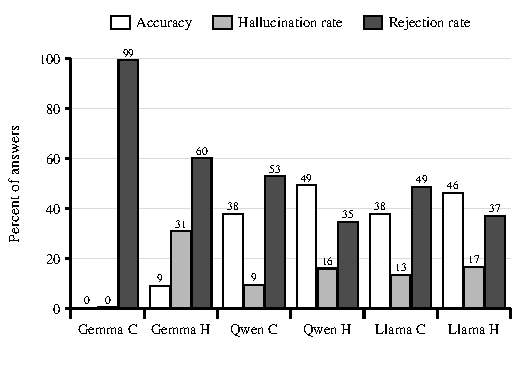
\includegraphics[width=\columnwidth]{figures/fig2.pdf}
\caption{End-to-end results reported in~\cite{mala_ml} (C = Contriever, H = Hybrid LI + Rerank). Hybrid retrieval raises accuracy and hallucination together for Qwen3-4B and Llama-3.1-8B, the trade-off that motivates claim-level verification.}
\label{fig:f2}
\end{figure}

\subsection{Experimental Results and Comparative Analysis}

Table VIII reports all methods on the 10,422 HaluBench test answers; every threshold is selected on the 4,466 development answers. Following the remark that the verifier must be improved before the gate can help, we first compare verifiers under uniform verification (B2), then the gate at matched budgets.

\begin{table*}[t]
\centering
\caption{Detection of unsupported answers on the full HaluBench test set (10,422 answers, 48.7\% unsupported). Thresholds selected on the development set ($\tau$ = 0.7 for NLI-base, 0.8 for NLI-large and HHEM, 0.55 for MiniCheck). The cheap stage costs 0.023 s per answer (0.028 s with the small NLI features of the revised method). Revised = 8 features, disagreement gate (Eq. (5)) and NLI-large. Verifier time = call rate $\times$ claims per answer (1.32) $\times$ seconds per claim. --- : not computed for that operating point.}
\label{tab:t8}
\footnotesize
\setlength{\tabcolsep}{3pt}
\renewcommand{\arraystretch}{1.12}
\begin{tabularx}{\textwidth}{>{\raggedright\arraybackslash\hsize=2.521\hsize}X>{\raggedright\arraybackslash\hsize=0.548\hsize}X>{\raggedright\arraybackslash\hsize=0.548\hsize}X>{\raggedright\arraybackslash\hsize=1.479\hsize}X>{\raggedright\arraybackslash\hsize=0.658\hsize}X>{\raggedright\arraybackslash\hsize=0.712\hsize}X>{\raggedright\arraybackslash\hsize=0.658\hsize}X>{\raggedright\arraybackslash\hsize=0.877\hsize}X}
\toprule
\textbf{Method} & \textbf{P} & \textbf{R} & \textbf{F1 [95\% CI]} & \textbf{AUROC} & \textbf{Macro-F1} & \textbf{Call rate} & \textbf{Verifier s / ans.} \\
\midrule
Flag every answer & 0.487 & 1.000 & 0.655 & 0.500 & 0.618 & 0 & 0 \\
B1 cheap only, 4 features (original) & 0.705 & 0.600 & 0.648 [0.637, 0.659] & 0.747 & 0.519 & 0 & 0 \\
B1 cheap only, 8 features (revised) & 0.689 & 0.646 & 0.667 [0.656, 0.677] & 0.744 & 0.566 & 0 & 0 \\
B2 uniform, NLI-base, top-4 premise & 0.571 & 0.808 & 0.669 [0.660, 0.678] & 0.697 & 0.629 & 1 & 0.021 \\
B2 uniform, NLI-large, top-4 premise & 0.746 & 0.761 & \textbf{0.753} [0.744, 0.762] & \textbf{0.816} & \textbf{0.660} & 1 & 0.019 \\
B2 uniform, MiniCheck, passage & 0.545 & 0.838 & 0.661 [0.652, 0.670] & 0.687 & 0.648 & 1 & 0.179 \\
B2 uniform, HHEM-2.1, passage & 0.602 & 0.816 & 0.693 [0.684, 0.702] & 0.749 & 0.657 & 1 & 0.072 \\
MiniCheck, answer level & 0.561 & 0.794 & 0.657 [0.648, 0.667] & 0.685 & 0.630 & 1 / ans. & 0.142 \\
HHEM-2.1, answer level & 0.622 & 0.788 & 0.695 [0.686, 0.705] & 0.754 & 0.666 & 1 / ans. & 0.059 \\
B3 original (NLI-base, $\theta$* = 0.999) & 0.706 & 0.602 & 0.650 [0.638, 0.661] & 0.747 & 0.520 & 0.002 & $<$0.001 \\
Revised, $\lambda$ = 0.3 ($\theta$* = 1) & 0.689 & 0.646 & 0.667 [0.656, 0.677] & 0.744 & 0.566 & 0 & 0 \\
Revised, $\lambda$ = 0.1 ($\theta$* = 0.7) & 0.738 & 0.726 & 0.732 & 0.734 & --- & 0.42 & 0.008 \\
Revised, $\lambda$ = 0.05 ($\theta$* = 0.625) & 0.738 & 0.744 & 0.741 & 0.737 & --- & 0.53 & 0.010 \\
\bottomrule
\end{tabularx}
\end{table*}

\textit{The verifier was the main weakness:} With the NLI-base model used in the first version, uniform verification (F1 0.669) is barely above flagging every answer (0.655). Replacing it by a larger NLI model trained on more inference data (DeBERTa-v3-large on MNLI, FEVER, ANLI, LingNLI and WANLI) raises F1 to 0.753 and AUROC to 0.816 at the same cost per call (paired bootstrap difference +0.084, 95\% CI [0.075, 0.093]; versus flag-all +0.098 [0.088, 0.107]). It also beats the trained factual-consistency detectors: HHEM-2.1 reaches 0.693--0.695 (+0.040 over flag-all) and MiniCheck 0.657--0.661 (+0.002, $p$ = 0.62), at 4--9 times the verifier time, because they read the whole passage. The two detectors have a better macro-F1 than NLI-base, and HHEM is the best method on RAGTruth (Table XIV), so no single verifier dominates on every source.

\textit{Why NLI rejected supported answers:} Uniform NLI-base flags 3,091 supported test answers. Of the 4,163 claims it rejects in them, 59.0\% are short answers wrapped in the template ``The answer to the question $q$ is $a$.'', which turns a correct span into a hypothesis that the premise rarely states literally; 5.1\% are claims whose content words occur in the passage but not in the four-sentence premise; and 35.9\% are model errors with the evidence present (mostly paraphrases and arithmetic, as in DROP). NLI-large rejects 1,913 claims in 1,317 supported answers, and the template share falls to 37.7\%: the larger model handles the template far better, which is the main source of its gain. The premise share rises to 8.7\%, so premise construction becomes relatively more important once the verifier is stronger. Calibrated thresholds are used throughout ($\tau$ is selected on the development set), and the always-unsupported baseline is the flag-all row.

\begin{figure*}[t]
\centering
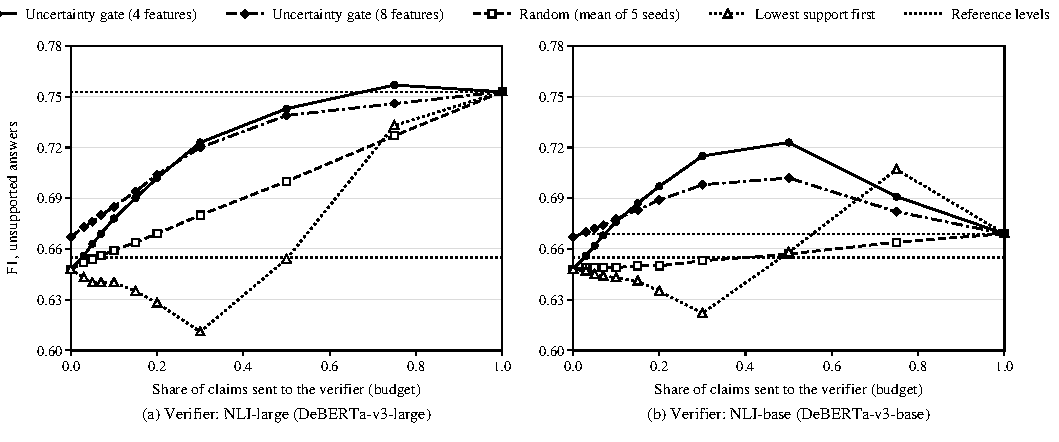
\includegraphics[width=\textwidth]{figures/fig3.pdf}
\caption{F1 on the HaluBench test set (10,422 answers) when a fixed share of all claims is sent to the verifier (matched budgets). Claims are ranked globally by each strategy's priority; random escalation is the mean of five seeds (SD $\le$ 0.004). Budget 0 is cheap-only verification (B1) and budget 1 is uniform verification (B2). Dotted reference levels: flagging every answer (F1 0.655) and uniform verification (0.753 with NLI-large, 0.669 with NLI-base). The disagreement gate coincides with the uncertainty gate within 0.002 and is not drawn. With NLI-large, latency grows from 0.023 s per answer at budget 0 to 0.042 s at budget 1.}
\label{fig:f3}
\end{figure*}

\textit{Selective escalation at matched budgets:} Because a threshold selected with one $\lambda$ hides the trade-off, Fig. 3 and Table IX compare escalation strategies at the same share of verified claims. Escalating the most uncertain claims is clearly better than escalating at random: at 10\% of the claims the uncertainty gate reaches F1 0.678 against 0.659, at 30\% 0.723 against 0.680 and at 50\% 0.743 against 0.700. Escalating 75\% of the claims gives F1 0.757, slightly above uniform verification (0.753), at three quarters of the cost. Escalating the claims with the lowest cheap support first, a confidence-based alternative, is worse than random up to a budget of 30\%, because those claims are already rejected correctly by the cheap stage. The gain over random is however modest at small budgets: with 10\% of the calls the gate recovers 29\% of the F1 gap between cheap-only and uniform verification, and with 30\% it recovers 71\%. The same ordering holds with NLI-base, where verifying everything is worse than verifying the uncertain half (0.669 at budget 1 against 0.723 at 0.5).

\begin{table}[t]
\centering
\caption{F1 at matched verifier budgets (share of claims escalated) on the HaluBench test set. Budget 0 (cheap only): 0.648 with 4 features, 0.667 with 8; budget 1 (uniform): 0.753 with NLI-large, 0.669 with NLI-base.}
\label{tab:t9}
\scriptsize
\setlength{\tabcolsep}{2pt}
\renewcommand{\arraystretch}{1.12}
\begin{tabularx}{\columnwidth}{>{\raggedright\arraybackslash\hsize=2.605\hsize}X>{\raggedright\arraybackslash\hsize=0.733\hsize}X>{\raggedright\arraybackslash\hsize=0.733\hsize}X>{\raggedright\arraybackslash\hsize=0.733\hsize}X>{\raggedright\arraybackslash\hsize=0.733\hsize}X>{\raggedright\arraybackslash\hsize=0.733\hsize}X>{\raggedright\arraybackslash\hsize=0.733\hsize}X}
\toprule
\textbf{Verifier / cheap stage / strategy} & \textbf{5\%} & \textbf{10\%} & \textbf{20\%} & \textbf{30\%} & \textbf{50\%} & \textbf{75\%} \\
\midrule
NLI-large / 4 feat. / uncertainty & 0.663 & 0.678 & 0.702 & 0.723 & 0.743 & 0.757 \\
NLI-large / 4 feat. / disagreement & 0.663 & 0.678 & 0.702 & 0.723 & 0.743 & 0.757 \\
NLI-large / 4 feat. / random & 0.654 & 0.659 & 0.669 & 0.680 & 0.700 & 0.727 \\
NLI-large / 4 feat. / lowest support & 0.640 & 0.640 & 0.628 & 0.611 & 0.654 & 0.733 \\
NLI-large / 8 feat. / uncertainty & 0.676 & 0.685 & 0.704 & 0.720 & 0.739 & 0.746 \\
NLI-large / 8 feat. / random & 0.671 & 0.676 & 0.684 & 0.692 & 0.708 & 0.731 \\
NLI-base / 4 feat. / uncertainty & 0.662 & 0.676 & 0.697 & 0.715 & 0.723 & 0.691 \\
NLI-base / 4 feat. / random & 0.649 & 0.649 & 0.650 & 0.653 & 0.657 & 0.664 \\
\bottomrule
\end{tabularx}
\end{table}

\begin{table}[t]
\centering
\caption{Operating point of the revised method (8 features, disagreement gate, NLI-large) selected on the development set for each price $\lambda$ of a verifier call (Eq. (1)), evaluated on the test set.}
\label{tab:t10}
\scriptsize
\setlength{\tabcolsep}{2pt}
\renewcommand{\arraystretch}{1.12}
\begin{tabularx}{\columnwidth}{>{\raggedright\arraybackslash\hsize=1.132\hsize}X>{\raggedright\arraybackslash\hsize=0.926\hsize}X>{\raggedright\arraybackslash\hsize=1.132\hsize}X>{\raggedright\arraybackslash\hsize=0.926\hsize}X>{\raggedright\arraybackslash\hsize=0.926\hsize}X>{\raggedright\arraybackslash\hsize=0.926\hsize}X>{\raggedright\arraybackslash\hsize=1.029\hsize}X}
\toprule
\textbf{$\lambda$} & \textbf{$\theta$*} & \textbf{Call rate} & \textbf{P} & \textbf{R} & \textbf{F1} & \textbf{AUROC} \\
\midrule
0 & 0.325 & 0.944 & 0.740 & 0.771 & 0.755 & 0.810 \\
0.05 & 0.625 & 0.535 & 0.738 & 0.744 & 0.741 & 0.737 \\
0.1 & 0.700 & 0.420 & 0.738 & 0.726 & 0.732 & 0.734 \\
0.2 & 0.875 & 0.167 & 0.719 & 0.678 & 0.698 & 0.741 \\
0.3, 0.5 & 1.000 & 0 & 0.689 & 0.646 & 0.667 & 0.744 \\
\bottomrule
\end{tabularx}
\end{table}

\textit{Trade-off over $\theta$ and $\lambda$:} Table X lists the operating point that Eq. (1) selects for each $\lambda$. With $\lambda$ = 0.3, the value used in the first version, the revised method selects $\theta$ = 1 and makes no call: once the cheap stage has 8 features, the expected F1 gain of a call is smaller than its price, and the method degenerates to cheap-only verification (F1 0.667; +0.017 over the original B3, CI [0.007, 0.026], and +0.011 over flag-all, CI [$-$0.0001, 0.023]). With $\lambda$ = 0.1 it verifies 42\% of the claims for F1 0.732, and with $\lambda$ = 0.05 53\% for 0.741. Lowering $\theta$ trades F1 for AUROC non-monotonically because the answer risk mixes cheap probabilities and verifier scores, which are on different scales. The choice of $\lambda$ is therefore a deployment decision; we report the whole curve rather than a single point.

\textit{Confidently wrong cheap predictions:} On the 9,330 single-claim test answers the cheap stage (4 features) makes 2,679 errors; 480 of them (17.9\%) are confident (|2$p$ $-$ 1| $\ge$ 0.5), so no uncertainty threshold below 0.5 sends them to the verifier. The disagreement term of Eq. (5) was meant to catch them, but it flags 0.6\% of the confident errors and 2.8\% of the confident correct predictions; with 8 features, 1.2\% against 0.9\%. A contradiction from the small NLI model is even less specific (28.8\% of confident errors against 38.1\% of confident correct predictions). The two cheap signals therefore err together, and the disagreement gate coincides with the uncertainty gate at every budget (Table IX). Catching confident errors needs a signal that is independent of the cheap features, such as the strong verifier itself.

\subsection{Ablation Studies and Additional Validation}

All ablations are compared at matched budgets, with NLI-large as verifier unless stated (Table XI). For the cheap stage we also report the AUROC and ECE of the calibrated probability on single-claim test answers.

\begin{table}[t]
\centering
\caption{Ablations on the HaluBench test set at matched budgets (uncertainty gate). AUROC and ECE of the calibrated support probability on single-claim answers. Premise rows use NLI-base and the 4-feature cheap stage.}
\label{tab:t11}
\scriptsize
\setlength{\tabcolsep}{2pt}
\renewcommand{\arraystretch}{1.12}
\begin{tabularx}{\columnwidth}{>{\raggedright\arraybackslash\hsize=2.059\hsize}X>{\raggedright\arraybackslash\hsize=0.988\hsize}X>{\raggedright\arraybackslash\hsize=0.659\hsize}X>{\raggedright\arraybackslash\hsize=0.947\hsize}X>{\raggedright\arraybackslash\hsize=0.782\hsize}X>{\raggedright\arraybackslash\hsize=0.782\hsize}X>{\raggedright\arraybackslash\hsize=0.782\hsize}X}
\toprule
\textbf{Variant} & \textbf{AUROC p} & \textbf{ECE} & \textbf{F1 cheap only} & \textbf{F1 @10\%} & \textbf{F1 @30\%} & \textbf{F1 @50\%} \\
\midrule
4 features (original) & 0.800 & 0.232 & 0.648 & 0.678 & 0.723 & 0.743 \\
8 features (revised) & 0.776 & 0.089 & 0.667 & 0.685 & 0.720 & 0.739 \\
8 without small NLI & 0.759 & 0.166 & 0.654 & 0.677 & 0.708 & 0.725 \\
8 without negation/number & 0.785 & 0.121 & 0.666 & 0.686 & 0.722 & 0.743 \\
Small NLI only & 0.673 & 0.022 & 0.551 & 0.588 & 0.662 & 0.722 \\
Similarity only & 0.558 & 0.016 & 0.453 & 0.494 & 0.564 & 0.631 \\
Raw similarity, no calibrator & 0.558 & 0.124 & 0.355 & 0.404 & 0.508 & 0.606 \\
Premise m = 1 (NLI-base) & --- & --- & 0.648 & 0.684 & 0.732 & 0.735 \\
Premise m = 2 (NLI-base) & --- & --- & 0.648 & 0.676 & 0.718 & 0.726 \\
Premise m = 4 (NLI-base) & --- & --- & 0.648 & 0.676 & 0.715 & 0.723 \\
Premise m = 8 (NLI-base) & --- & --- & 0.648 & 0.676 & 0.714 & 0.720 \\
Evidence chain (NLI-base) & --- & --- & 0.648 & 0.676 & 0.716 & 0.723 \\
\bottomrule
\end{tabularx}
\end{table}

\textit{Cheap stage:} Calibration and coverage features matter: the similarity feature alone reaches F1 0.453 without escalation and raw similarity 0.355, against 0.648 for the calibrated four-feature model. The contradiction-sensitive features improve the F1 of the cheap stage (0.648 $\rightarrow$ 0.667) and macro-F1 (0.519 $\rightarrow$ 0.566) and cut the ECE from 0.232 to 0.089, but they slightly lower the AUROC of the claim probability (0.800 $\rightarrow$ 0.776) and give no gain once claims are escalated (0.720 against 0.723 at 30\%). Removing the small NLI features costs most (0.708 at 30\%); removing negation and number mismatch changes nothing. \textbf{Premise.} On HaluBench, whose passages are short and whose questions are mostly single-hop, the single most similar sentence is the best premise for NLI-base (0.732 at 30\%), and neither longer top-$m$ premises nor the evidence chain help; the multi-hop test below gives a different picture.

\begin{table}[t]
\centering
\caption{Claim-level evaluation on HaluBench with claim labels from an LLM judge (Qwen2.5-7B-Instruct; 300 development and 600 test claims from multi-claim and single-claim answers, 48.5\% unsupported).}
\label{tab:t12}
\footnotesize
\setlength{\tabcolsep}{3pt}
\renewcommand{\arraystretch}{1.12}
\begin{tabularx}{\columnwidth}{>{\raggedright\arraybackslash\hsize=1.692\hsize}X>{\raggedright\arraybackslash\hsize=1.026\hsize}X>{\raggedright\arraybackslash\hsize=0.410\hsize}X>{\raggedright\arraybackslash\hsize=0.872\hsize}X}
\toprule
\textbf{Model or verifier} & \textbf{Claim AUROC} & \textbf{ECE} & \textbf{Claim F1} \\
\midrule
Calibrator, 4 feat., answer labels & 0.647 & 0.057 & 0.589 \\
Calibrator, 4 feat., claim labels & 0.689 & 0.037 & 0.595 \\
Calibrator, 8 feat., answer labels & 0.672 & 0.072 & 0.619 \\
Calibrator, 8 feat., claim labels & 0.727 & 0.062 & 0.653 \\
NLI-base, top-1 / top-4 / top-8 & 0.633 / 0.732 / 0.722 & --- & 0.681 / 0.703 / 0.694 \\
NLI-base, evidence chain & 0.697 & --- & 0.672 \\
NLI-large, top-4 / chain & 0.745 / 0.729 & --- & 0.682 / 0.690 \\
MiniCheck, passage & 0.764 & --- & 0.728 \\
HHEM-2.1, passage & 0.770 & --- & 0.717 \\
\bottomrule
\end{tabularx}
\end{table}

\textit{Claim-level labels and the calibration mismatch:} The calibrator of the first version is trained on single-claim answers, whose claim label equals the answer label, but applied to every claim. To measure the mismatch we labelled 900 claims with an open-weight LLM judge; on single-claim answers the judge agrees with the HaluBench label in 68\% of cases, so these are silver labels, and 150 claims are exported for manual annotation. Training on claim labels raises the claim-level AUROC from 0.647 to 0.689 (4 features) and from 0.672 to 0.727 (8 features) and lowers the ECE, confirming the mismatch; the eight-feature calibrator trained on claim labels is the best cheap model. At the claim level the trained consistency models rank best (AUROC 0.764--0.770), ahead of NLI-large (0.745), the opposite of the answer level; with an imperfect judge this difference should be confirmed on the manual labels.

\textit{Claim extraction:} 89.5\% of the test answers yield one claim, and the mean is 1.32 (RAGTruth 5.33, PubMedQA 1.75). The eight-claim cap is reached by 145 answers (1.4\%), 52 of them unsupported, and none of these is unsupported only because of a claim beyond the cap. On 300 multi-sentence answers, LLM decomposition into atomic facts gives 4.50 claims per answer against 3.07 for the rule-based extractor, with the same share of unsupported claims (0.330 against 0.337) and the same answer-level detection with uniform NLI-large (F1 0.608 against 0.611, AUROC 0.647 against 0.641). On this benchmark atomic decomposition therefore adds cost without changing detection; most HaluBench answers are already atomic.

\begin{table*}[t]
\centering
\caption{Multi-hop claims (HotpotQA validation, 1,400 test claims, 50\% unsupported with hard wrong answers): share of premises that contain evidence from both supporting documents, premise length, and claim-level AUROC of each verifier. Gold: the annotated supporting sentences (oracle).}
\label{tab:t13}
\footnotesize
\setlength{\tabcolsep}{3pt}
\renewcommand{\arraystretch}{1.12}
\begin{tabularx}{\textwidth}{>{\raggedright\arraybackslash\hsize=1.765\hsize}X>{\raggedright\arraybackslash\hsize=0.824\hsize}X>{\raggedright\arraybackslash\hsize=0.647\hsize}X>{\raggedright\arraybackslash\hsize=0.824\hsize}X>{\raggedright\arraybackslash\hsize=0.824\hsize}X>{\raggedright\arraybackslash\hsize=0.824\hsize}X>{\raggedright\arraybackslash\hsize=0.706\hsize}X>{\raggedright\arraybackslash\hsize=1.588\hsize}X}
\toprule
\textbf{Premise} & \textbf{Both docs} & \textbf{Words} & \textbf{NLI-base} & \textbf{NLI-large} & \textbf{MiniCheck} & \textbf{HHEM} & \textbf{NLI-large bridge / comp.} \\
\midrule
Top-1 sentence & 0.000 & 22 & 0.473 & 0.649 & --- & --- & 0.651 / 0.645 \\
Top-2 & 0.192 & 44 & 0.560 & 0.736 & --- & --- & 0.747 / 0.680 \\
Top-4 & 0.404 & 89 & 0.605 & 0.785 & 0.616 & 0.618 & 0.796 / 0.724 \\
Top-8 & 0.630 & 180 & 0.563 & \textbf{0.822} & --- & --- & 0.842 / 0.722 \\
Evidence chain & 0.337 & 68 & 0.595 & 0.766 & 0.591 & 0.605 & 0.777 / 0.710 \\
All 10 paragraphs & 1.000 & --- & --- & --- & 0.575 & 0.599 & --- \\
Gold supporting sentences & 1.000 & --- & 0.757 & 0.927 & 0.759 & 0.729 & 0.945 / 0.817 \\
\bottomrule
\end{tabularx}
\end{table*}

\textit{Multi-hop claims that need two documents (E3):} Table XIII uses 1,400 HotpotQA claims with exact labels whose verification needs the two supporting documents among ten paragraphs. Premise construction is the bottleneck: with the gold supporting sentences NLI-large reaches AUROC 0.927, but with the four most similar sentences only 0.785, because 60\% of these premises miss one of the two documents. A single sentence never covers both (AUROC 0.649). Coverage, not length, drives accuracy: top-8 premises cover both documents in 63\% of cases and give the best AUROC (0.822). The evidence chain covers both documents less often than top-4 (34\% against 40\%) with 24\% fewer words, and is slightly worse (0.766); its hop-2 rule, which prefers bridge terms from a different document, often lands in a distractor paragraph that shares the bridge entity. Comparison questions are harder than bridge questions for every premise. MiniCheck and HHEM, run on the same premises, are far behind NLI-large (0.58--0.62), and reading all ten paragraphs does not help them, because the distractors contain the wrong answers. The cheap stage cannot separate these claims (AUROC 0.566 with claim labels, 0.546 with 8 features): every wrong answer is an entity or number that appears in the context, which is exactly what the coverage features reward. Consequently the gate is only useful at large budgets here (F1 with NLI-large and top-4 premises: 0.267 cheap only, 0.502 at 30\%, 0.618 at 50\%, 0.759 uniform).

\begin{table*}[t]
\centering
\caption{F1 by HaluBench source on the test set. B1 and the original B3 coincide (B3 escalates 0.2\% of claims).}
\label{tab:t14}
\footnotesize
\setlength{\tabcolsep}{3pt}
\renewcommand{\arraystretch}{1.12}
\begin{tabularx}{\textwidth}{>{\raggedright\arraybackslash\hsize=1.412\hsize}X>{\raggedright\arraybackslash\hsize=0.588\hsize}X>{\raggedright\arraybackslash\hsize=0.824\hsize}X>{\raggedright\arraybackslash\hsize=1.059\hsize}X>{\raggedright\arraybackslash\hsize=1.235\hsize}X>{\raggedright\arraybackslash\hsize=1.118\hsize}X>{\raggedright\arraybackslash\hsize=0.941\hsize}X>{\raggedright\arraybackslash\hsize=0.824\hsize}X}
\toprule
\textbf{Source} & \textbf{n} & \textbf{Flag all} & \textbf{B1 / B3 orig.} & \textbf{Revised ($\lambda$ = 0.3)} & \textbf{B2 NLI-large} & \textbf{MiniCheck} & \textbf{HHEM} \\
\midrule
DROP & 697 & \textbf{0.676} & 0.367 & 0.377 & 0.522 & 0.642 & 0.669 \\
FinanceBench & 700 & \textbf{0.679} & 0.657 & 0.657 & 0.627 & 0.672 & 0.673 \\
RAGTruth & 625 & 0.329 & 0.365 & 0.375 & 0.383 & 0.443 & \textbf{0.608} \\
CovidQA & 700 & 0.674 & 0.343 & 0.590 & \textbf{0.896} & 0.664 & 0.652 \\
HaluEval & 7,000 & 0.670 & 0.729 & 0.731 & \textbf{0.822} & 0.664 & 0.709 \\
PubMedQA & 700 & 0.677 & 0.654 & 0.665 & \textbf{0.708} & 0.696 & 0.687 \\
\bottomrule
\end{tabularx}
\end{table*}

\textit{Per-source errors and calibration:} Table XIV shows that the cheap stage fails on DROP (F1 0.367), CovidQA (0.343; precision 0.926 but recall 0.211) and RAGTruth, and that no method beats flag-all on DROP and FinanceBench, whose hallucinations often need arithmetic over numbers or tables. NLI-large solves CovidQA (0.896) and HaluEval (0.822), and HHEM is clearly best on the long answers of RAGTruth (0.608). We attributed every wrong decision of the gated methods to the first stage that explains it (extraction, evidence missing from the premise, a confident or a borderline cheap error, or the verifier). Because B3 and the revised method at $\lambda$ = 0.3 almost never escalate, all their errors are cheap-stage errors; borderline errors dominate on HaluEval (1,433 against 106 confident), CovidQA (287 borderline) and DROP, and confident errors on FinanceBench (287); extraction causes 4 errors (RAGTruth). A separate calibrator per source, fitted on that source's development answers and applied to unseen test answers, raises micro-F1 (4 features: 0.648 $\rightarrow$ 0.720; 8 features: 0.667 $\rightarrow$ 0.739) and AUROC (0.747 $\rightarrow$ 0.840), mainly by adapting the decision boundary to HaluEval, but lowers macro-F1 (0.519 $\rightarrow$ 0.515; 0.566 $\rightarrow$ 0.552). It helps the dominant source rather than the hard ones, so we keep a global calibrator; per-source calibration also requires knowing the source at test time.

\subsection{End-to-End Verification on HotpotQA Answers}

The final step of the reproduction, labelling the 3,600 generated Qwen3-4B answers with the judge and applying the verifier to them before and after filtering, could not be completed within the free GPU budget of this study: the required session waited more than three hours in the shared GPU queue without starting and was cancelled. We therefore report no end-to-end accuracy, hallucination rate or claim-level faithfulness for these answers, and we do not claim an answer to RQ1. The generated answers, the judge and the complete evaluation script are released with the code, so that the experiment can be run with one command on any GPU with at least 8 GB of memory. The controlled multi-hop experiment of Section IV-E, whose labels are exact, is the evidence this paper offers for the multi-hop setting.

\section{Discussion}

The study began from a simple premise: if a cheap model can tell which claims are clearly supported or clearly unsupported, an expensive verifier needs to examine only the rest. The first version of the method appeared to refute that premise, because the adaptive verifier was barely better than flagging every answer. The revised experiments show that this failure had a different cause. The verifier itself, not the gate, was the weak component. An inference model that rejected most correct short answers once they were rewritten as hypotheses could not reward any routing strategy, however well calibrated. Once a stronger inference model replaced it, uniform verification rose well above the trivial reference and above two detectors trained specifically for factual consistency, while the cost per call stayed the same.

With a verifier that carries real information, the question of selective verification becomes meaningful again, and the matched-budget comparison answers it more clearly than any single operating point could. Sending the claims on which the cheap model is least certain to the verifier is consistently better than sending a random share of the same size, and it is much better than sending the claims with the lowest cheap support, which the cheap stage already rejects correctly. Three quarters of the verification budget suffices to match uniform verification. The savings at small budgets, however, are moderate, and the cost-weighted selection rule turns this into a practical caveat: once the cheap stage improved, the price of a call used in the first version made the method decline to verify at all. The cost of verification is therefore a deployment choice that must be made explicitly, and reporting the whole trade-off curve is more informative than reporting the point chosen by one price.

The analysis of confidently wrong cheap predictions explains why the remaining gap is hard to close. About one fifth of the cheap-stage errors are made with high confidence, and no uncertainty threshold can route them to the verifier. The disagreement signal was introduced for exactly these cases, but the small inference model and the calibrated probability tend to fail on the same claims, so their disagreement is rare where it would matter. Contradiction-sensitive features improved the calibration and the cheap-only accuracy, yet they did not make the gate better at choosing what to escalate. A signal that is independent of the cheap features, for example a learned predictor of where the verifier would change the decision, appears necessary for a cheap stage to catch its own confident mistakes.

The multi-hop experiments shift attention from the verifier to the evidence it reads. When the verifier is given the two annotated supporting sentences, it separates supported from unsupported multi-hop claims almost perfectly; when it is given the sentences most similar to the claim, it frequently sees only one of the two documents, and its accuracy drops accordingly. Wider premises that cover more documents recover much of this loss, whereas the evidence chain, which tries to follow a bridge entity, is drawn into distractor paragraphs that share that entity. On the same claims the cheap stage is nearly blind, because every wrong answer in this setting is an entity or number that does appear in the context, which is precisely what coverage features reward. For multi-hop retrieval-augmented generation, the evidence presented to the verifier is therefore at least as important as the verifier, and selective verification can save only what the cheap stage is able to recognize.

These conclusions are bounded by several limitations. Support is measured against the retrieved context, not against world knowledge. Claim labels on HaluBench and answer labels on HotpotQA come from an open-weight judge with seven billion parameters instead of the commercial judge of the base study, and that judge agrees with the HaluBench labels on 68\% of single-claim answers; the 150 claims exported for manual annotation have not yet been labelled. Only one of the three generators of the base study was run, because the other two require gated access, and the answers it generated were not yet labelled and verified end to end. The multi-hop claims are constructed from gold answers and distractor entities and are cleaner than generated text. Finally, the answer-level decision takes the maximum over claims, which inflates false alarms on long answers, and the inference models read at most 512 tokens, so longer evidence must be split into chunks.

\section{Conclusion}

This work set out to detect unsupported claims in retrieval-augmented answers without paying for full verification of every claim. We reimplemented the faithfulness benchmark of~\cite{mala_ml} and showed with controlled variants that the gap between its printed retrieval scores and the authors' public code arises mostly from question-scoped document identifiers that count duplicate sentences as non-relevant, not from the metric implementation. On the full HaluBench test set, the decisive improvement came from the verifier: uniform verification with a large natural-language-inference model reached an F1 of 0.753 and an AUROC of 0.816, ahead of HHEM-2.1 and MiniCheck, after the original model had been shown to fail mainly on correct short answers rewritten as hypotheses. Escalating the most uncertain claims outperformed random and confidence-based escalation at every matched budget and matched uniform verification with three quarters of the calls, while the proposed disagreement signal brought no further gain. On multi-hop claims, premise coverage of all supporting documents emerged as the main bottleneck.

Future work follows directly from these findings. The most immediate step is to label and verify the 3,600 generated HotpotQA answers, which completes the reproduction and measures claim-level faithfulness before and after verification under sparse, dense and hybrid retrieval. Premises for multi-hop claims should guarantee coverage of every retrieved document, for instance by taking one sentence per document or by letting the verifier drive an iterative chain; the gate should be trained on where the verifier changes the decision, with a signal independent of the cheap features; and human claim-level labels are needed to settle the comparison between inference and consistency models. We also plan to run the two remaining generators, evaluate a generative hallucination judge on larger hardware, extend the evaluation to MuSiQue and 2WikiMultiHopQA, and replace the deletion of unsupported claims with evidence-grounded rewriting.

\section*{Data and Code Availability}

All datasets used in this study are publicly available from the sources below; the access dates refer to the downloads used for the reported runs.

\textbullet{} HotpotQA (distractor setting) --- \url{https://huggingface.co/datasets/hotpotqa/hotpot_qa} (accessed 23 Nov. 2026)

\textbullet{} HotpotQA project page --- \url{https://hotpotqa.github.io} (accessed 23 Nov. 2026)

\textbullet{} HaluBench --- \url{https://huggingface.co/datasets/PatronusAI/HaluBench} (accessed 23 Nov. 2026)

\textbullet{} Base benchmark repository~\cite{mala_ml} --- \url{https://github.com/chandanasreemala/Beyond_Retrieval} (accessed 23 Nov. 2026)

\textbullet{} Code of this study --- \url{https://github.com/iqrafarooq-7839/adaptive-claim-verification-rag} (accessed 24 Nov. 2026)

\begin{thebibliography}{00}
\bibitem{huang_tois} L. Huang, W. Yu, W. Ma, W. Zhong, Z. Feng, H. Wang, Q. Chen, W. Peng, X. Feng, B. Qin, and T. Liu, ``A survey on hallucination in large language models: Principles, taxonomy, challenges, and open questions,'' \textit{ACM Trans. Inf. Syst.}, vol. 43, no. 2, pp. 1--55, 2025, doi: 10.1145/3703155.
\bibitem{cheng_tois} M. Cheng, Y. Luo, J. Ouyang, Q. Liu, H. Liu, L. Li, S. Yu, B. Zhang, J. Cao, J. Ma, D. Wang, and E. Chen, ``A survey on knowledge-oriented retrieval-augmented generation,'' \textit{ACM Trans. Inf. Syst.}, vol. 44, no. 8, pp. 1--57, 2026, doi: 10.1145/3833415.
\bibitem{huang_csur} Y. Huang and J. X. Huang, ``A survey on retrieval-augmented text generation for large language models,'' \textit{ACM Comput. Surv.}, vol. 58, no. 12, pp. 1--38, 2026, doi: 10.1145/3805774.
\bibitem{zhu_tois} Y. Zhu, H. Yuan, S. Wang, J. Liu, W. Liu, C. Deng, H. Chen, Z. Liu, Z. Dou, and J.-R. Wen, ``Large language models for information retrieval: A survey,'' \textit{ACM Trans. Inf. Syst.}, vol. 44, no. 1, pp. 1--54, 2025, doi: 10.1145/3748304.
\bibitem{ni_csur} B. Ni, Z. Liu, Y. Lei, L. Wang, Y. Zhao, X. Cheng, Q. Zeng, X. Dong, Y. Xia, K. Kenthapadi, R. Rossi, F. Dernoncourt, M. Tanjim, N. Ahmed, X. Liu, W. Fan, E. Blasch, Y. Wang, M. Jiang, and T. Derr, ``Towards trustworthy retrieval augmented generation for large language models: A survey,'' \textit{ACM Comput. Surv.}, vol. 58, no. 15, pp. 1--36, 2026, doi: 10.1145/3837074.
\bibitem{peng_tois} B. Peng, Y. Zhu, Y. Liu, X. Bo, H. Shi, C. Hong, Y. Zhang, and S. Tang, ``Graph retrieval-augmented generation: A survey,'' \textit{ACM Trans. Inf. Syst.}, vol. 44, no. 2, pp. 1--52, 2025, doi: 10.1145/3777378.
\bibitem{mala_ml} C. S. Mala, G. Gezici, and F. Giannotti, ``Disentangling faithfulness hallucinations in retrieval-augmented generation: A systematic benchmark and analysis,'' \textit{Mach. Learn.}, vol. 115, no. 8, Art. no. 187, 2026, doi: 10.1007/s10994-026-07121-y.
\bibitem{huang_tkdd} Y. Huang, L. Yang, X.-H. Yang, and X. Xu, ``Retrieval-augmented generation for multi-hop question answering based on structured planning,'' \textit{ACM Trans. Knowl. Discov. Data}, vol. 20, no. 3, pp. 1--20, 2026, doi: 10.1145/3789506.
\bibitem{yuan_jksu} M. Yuan, T. Wang, and Y. Qian, ``AdaKG-RAG: Adaptive KG-guided retrieval-augmented generation with hypothesis-and-verification retrieval for multi-hop question answering,'' \textit{J. King Saud Univ. Comput. Inf. Sci.}, vol. 38, no. 6, Art. no. 605, 2026, doi: 10.1007/s44443-026-01028-3.
\bibitem{linders_ai} J. Linders and J. M. Tomczak, ``Knowledge graph-extended retrieval augmented generation for question answering,'' \textit{Appl. Intell.}, vol. 55, no. 17, Art. no. 1102, 2025, doi: 10.1007/s10489-025-06885-5.
\bibitem{wu_ml} J. Wu, J. Li, Z. Ning, and L. Wang, ``From relevance to utility: Faith-Rank for utility-driven evidence re-ranking and reliable answering in retrieval-augmented generation,'' \textit{Mach. Learn.}, vol. 115, no. 8, Art. no. 191, 2026, doi: 10.1007/s10994-026-07109-8.
\bibitem{kirubavathi_sr} G. Kirubavathi, M. Gopi, and K. S. Vidhun, ``VG-RAG: Verification-gated retrieval-augmented generation,'' \textit{Sci. Rep.}, published online Sep. 11, 2026, doi: 10.1038/s41598-026-67853-8.
\bibitem{sinha_tois} A. Sinha and K. Chakma, ``Adaptive query performance prediction for retrieval-augmented generation: Bridging retrieval quality and generation relevance,'' \textit{ACM Trans. Inf. Syst.}, vol. 44, no. 6, pp. 1--56, 2026, doi: 10.1145/3827605.
\bibitem{min_factscore} S. Min, K. Krishna, X. Lyu, M. Lewis, W.-t. Yih, P. Koh, M. Iyyer, L. Zettlemoyer, and H. Hajishirzi, ``FActScore: Fine-grained atomic evaluation of factual precision in long form text generation,'' in \textit{Proc. Conf. Empirical Methods in Natural Language Processing (EMNLP)}, 2023, pp. 12076--12100, doi: 10.18653/v1/2023.emnlp-main.741.
\bibitem{laban_summac} P. Laban, T. Schnabel, P. N. Bennett, and M. A. Hearst, ``SummaC: Re-visiting NLI-based models for inconsistency detection in summarization,'' \textit{Trans. Assoc. Comput. Linguist.}, vol. 10, pp. 163--177, 2022, doi: 10.1162/tacl\_a\_00453.
\bibitem{zha_alignscore} Y. Zha, Y. Yang, R. Li, and Z. Hu, ``AlignScore: Evaluating factual consistency with a unified alignment function,'' in \textit{Proc. 61st Annu. Meeting Assoc. Comput. Linguist. (ACL)}, 2023, pp. 11328--11348, doi: 10.18653/v1/2023.acl-long.634.
\bibitem{tang_minicheck} L. Tang, P. Laban, and G. Durrett, ``MiniCheck: Efficient fact-checking of LLMs on grounding documents,'' in \textit{Proc. Conf. Empirical Methods in Natural Language Processing (EMNLP)}, 2024, pp. 8818--8847, doi: 10.18653/v1/2024.emnlp-main.499.
\bibitem{vectara_hhem} Vectara, ``HHEM-2.1-Open: Hughes hallucination evaluation model,'' Hugging Face model card, 2024. [Online]. Available: \url{https://huggingface.co/vectara/hallucination_evaluation_model}
\bibitem{qian_vericite} H. Qian, Y. Fan, J. Guo, R. Zhang, Q. Chen, D. Yin, and X. Cheng, ``VeriCite: Towards reliable citations in retrieval-augmented generation via rigorous verification,'' in \textit{Proc. Annu. Int. ACM SIGIR Conf. Research and Development in Information Retrieval in the Asia Pacific Region (SIGIR-AP)}, 2025, pp. 47--54, doi: 10.1145/3767695.3769505.
\bibitem{pal_dai} A. Pal, ``Improving reliability of large language models via claim-level self-verification and uncertainty calibration,'' \textit{Discov. Artif. Intell.}, vol. 6, no. 1, Art. no. 1132, 2026, doi: 10.1007/s44163-026-02240-w.
\bibitem{jiang_flare} Z. Jiang, F. Xu, L. Gao, Z. Sun, Q. Liu, J. Dwivedi-Yu, Y. Yang, J. Callan, and G. Neubig, ``Active retrieval augmented generation,'' in \textit{Proc. Conf. Empirical Methods in Natural Language Processing (EMNLP)}, 2023, pp. 7969--7992, doi: 10.18653/v1/2023.emnlp-main.495.
\bibitem{manakul_selfcheck} P. Manakul, A. Liusie, and M. Gales, ``SelfCheckGPT: Zero-resource black-box hallucination detection for generative large language models,'' in \textit{Proc. Conf. Empirical Methods in Natural Language Processing (EMNLP)}, 2023, pp. 9004--9017, doi: 10.18653/v1/2023.emnlp-main.557.
\bibitem{sun_rearter} Z. Sun, Q. Wang, W. Yu, X. Zang, K. Zheng, J. Xu, X. Zhang, Y. Song, and H. Li, ``ReARTeR: Retrieval-augmented reasoning with trustworthy process rewarding,'' in \textit{Proc. 48th Int. ACM SIGIR Conf. Research and Development in Information Retrieval (SIGIR)}, 2025, pp. 1251--1261, doi: 10.1145/3726302.3730102.
\bibitem{wallat_ictir} J. Wallat, M. Heuss, M. de Rijke, and A. Anand, ``Correctness is not faithfulness in retrieval augmented generation attributions,'' in \textit{Proc. Int. ACM SIGIR Conf. Innovative Concepts and Theories in Information Retrieval (ICTIR)}, 2025, pp. 22--32, doi: 10.1145/3731120.3744592.
\bibitem{yang_hotpot} Z. Yang, P. Qi, S. Zhang, Y. Bengio, W. Cohen, R. Salakhutdinov, and C. D. Manning, ``HotpotQA: A dataset for diverse, explainable multi-hop question answering,'' in \textit{Proc. Conf. Empirical Methods in Natural Language Processing (EMNLP)}, 2018, pp. 2369--2380, doi: 10.18653/v1/D18-1259.
\bibitem{rahman_air} S. S. Rahman, M. A. Islam, M. M. Alam, M. Zeba, M. A. Rahman, S. S. Chowa, M. A. K. Raiaan, and S. Azam, ``Hallucination to truth: A review of fact-checking and factuality evaluation in large language models,'' \textit{Artif. Intell. Rev.}, vol. 59, no. 2, Art. no. 70, 2026, doi: 10.1007/s10462-025-11454-w.
\bibitem{naser_lre} M. Z. Naser, ``Hallucinations in generative artificial intelligence and large language models: Tests, datasets, detection and correction methods,'' \textit{Lang. Resour. Eval.}, vol. 60, no. 3, Art. no. 64, 2026, doi: 10.1007/s10579-026-09938-4.
\end{thebibliography}

\end{document}
